% =============================================================================
% Section 6.4: Future Work
% =============================================================================

\section{Future Work}
\label{sec:future-work}

While NexaLearn achieves its stated objectives, several enhancements would significantly extend its capabilities, scalability, and adoption potential. This section outlines ten specific directions for future development, ordered by estimated impact.

\subsection{Microservices Extraction}

The most impactful architectural enhancement is extracting the AI Pipeline and Payments modules into separate microservices. These are the two contexts with the highest CPU and I/O demands: AI pipeline callbacks involve LLM API calls that can take 5--30 seconds, and payment webhook processing has strict latency requirements. Extracting them would:

\begin{itemize}
  \item Allow independent horizontal scaling: the AI pipeline could run on GPU-equipped instances while the rest of the system remains on general-purpose compute.
  \item Isolate failure domains: a crash in the AI pipeline would not affect the ability to process payments or serve course content.
  \item Enable independent deployment cycles: the AI pipeline evolves faster (new models, prompt engineering) than the core course management context.
\end{itemize}

The extraction would follow the strangler fig pattern: the existing outbox events already provide the communication contract. A gRPC-based query service would replace the current in-process repository calls for synchronous queries (e.g., checking if a course exists before creating a payment intent).

\subsection{WebSocket-Based Real-Time Features}

Adding WebSocket support via NestJS's \texttt{Gateway} abstraction would unlock several features:

\begin{itemize}
  \item \textbf{Real-time notifications.} Learners receive instant alerts when a new quiz is published, a discussion reply is posted, or their AI-generated quiz is ready for review.
  \item \textbf{Live Q\&A sessions.} Instructors can host real-time question-and-answer sessions during live lectures, with upvoting and moderation.
  \item \textbf{Collaborative note-taking.} Multiple learners editing the same lesson note see each other's changes in real time via operational transformation or Conflict-Free Replicated Data Types (CRDTs).
\end{itemize}

The WebSocket layer would use Redis Pub/Sub for horizontal scalability: each application instance subscribes to a Redis channel and broadcasts messages to its connected clients. This avoids the sticky-session requirement of a naive WebSocket deployment.

\subsection{Redis-Backed Distributed Rate Limiting}

The current chat rate limiter stores counters in application memory, which works only in single-instance deployments. Moving to a Redis-backed implementation---using \texttt{INCR} with \texttt{EXPIRE}---would enforce global rate limits across all instances. The \texttt{@nestjs/throttler} package's \texttt{ThrottlerStorageRedisService} provides a drop-in replacement requiring minimal code changes.

\subsection{OAuth2 Social Login}

Adding OAuth2 providers---Google, GitHub, Facebook, and Microsoft---would reduce sign-up friction and align with the authentication expectations of modern web applications. The implementation would extend the Auth module with a new \texttt{SocialLoginService} that validates the OAuth2 token received from the provider, creates or links a local user account, and issues NexaLearn JWT tokens. Passport.js strategies (\texttt{passport-google-oauth20}, \texttt{passport-github2}) integrate naturally with NestJS's authentication framework.

\subsection{Course Recommendation Engine}

A basic collaborative-filtering recommendation engine would suggest courses to learners based on the completion behaviour of similar users. The implementation would:

\begin{enumerate}
  \item Compute a user--course interaction matrix from the Enrollment and Progress tables (implicit feedback: completed lessons, time spent, quiz scores).
  \item Apply matrix factorisation (e.g., alternating least squares) to generate embeddings for users and courses.
  \item Return the top-$k$ courses with the highest cosine similarity to the user's embedding vector.
\end{enumerate}

A simpler alternative suitable for the current architecture is a rule-based engine that recommends courses in the same category as previously completed courses, filtered by difficulty level and instructor rating.

\subsection{Multi-Tenant Support}

The current database schema includes a \texttt{Tenant} model that is referenced by \texttt{User} and \texttt{Course}, but the multi-tenant isolation layer is not fully implemented. True multi-tenancy would require:

\begin{itemize}
  \item Row-level security policies in PostgreSQL that automatically filter queries by \texttt{tenant\_id}.
  \item Tenant-aware caching keys in Redis (\texttt{cache:<tenant\_id>:<key>}).
  \item Tenant provisioning and deprovisioning workflows in a new \texttt{Admin} context.
  \item Per-tenant configuration (storage limits, rate limits, feature flags).
\end{itemize}

Multi-tenancy is the most requested feature from the university and corporate segments identified in Chapter~2. It would allow NexaLearn to operate as a SaaS platform serving multiple institutions from a single deployment.

\subsection{Certificate Blockchain Verification}

Digital certificates issued by the Certificates context could be anchored to a blockchain for tamper-evident verification. A SHA-256 hash of the certificate data (learner name, course name, completion date) would be submitted to a smart contract on a public blockchain (e.g., Ethereum or Polygon). Employers could verify a certificate by comparing the hash stored on-chain against the certificate presented by the learner. This feature has no direct revenue impact but would significantly differentiate NexaLearn from proprietary LMS platforms in the university segment.

\subsection{Mobile Push Notifications}

Adding push notification support via Firebase Cloud Messaging (FCM) for Android and Apple Push Notification Service (APNS) for iOS would allow the Notifications context to reach learners outside the web application. The implementation would:

\begin{enumerate}
  \item Add a \texttt{Device} entity to the Auth context that stores the platform type (iOS/Android) and the push token.
  \item Extend the \texttt{NotificationService} to send push notifications alongside email notifications.
  \item Handle token rotation, expired tokens, and unregister events.
\end{enumerate}

\subsection{React/Next.js Frontend}

The current project delivers only the backend API. Building a modern frontend application using React with Next.js would provide a reference implementation that demonstrates the API's capabilities. Priority pages include:

\begin{itemize}
  \item Course catalogue with search and filtering.
  \item Lesson viewer with embedded video player (HLS.js) and progress tracking.
  \item Quiz interface with multiple-choice, short-answer, and instant feedback.
  \item Instructor dashboard with course metrics and quiz analytics.
  \item Admin panel for user management and platform configuration.
\end{itemize}

The frontend would use Next.js App Router with server components for initial page load performance, client components for interactive elements, and React Query for server state management.

\subsection{GraphQL API Layer}

Alongside the existing REST API, a GraphQL endpoint would provide flexible data fetching for frontend clients. The NestJS \texttt{@nestjs/graphql} package supports a code-first approach where TypeScript classes decorated with \texttt{@ObjectType()} and \texttt{@Resolver()} generate the GraphQL schema automatically. A GraphQL layer would reduce over-fetching (restricting the discussion index to only thread titles) and under-fetching (loading a course with all modules, lessons, and instructor details in a single query). The existing DDD service layer can be reused directly; GraphQL resolvers would delegate to the same application services used by REST controllers.

\begin{figure}[H]
  \centering
  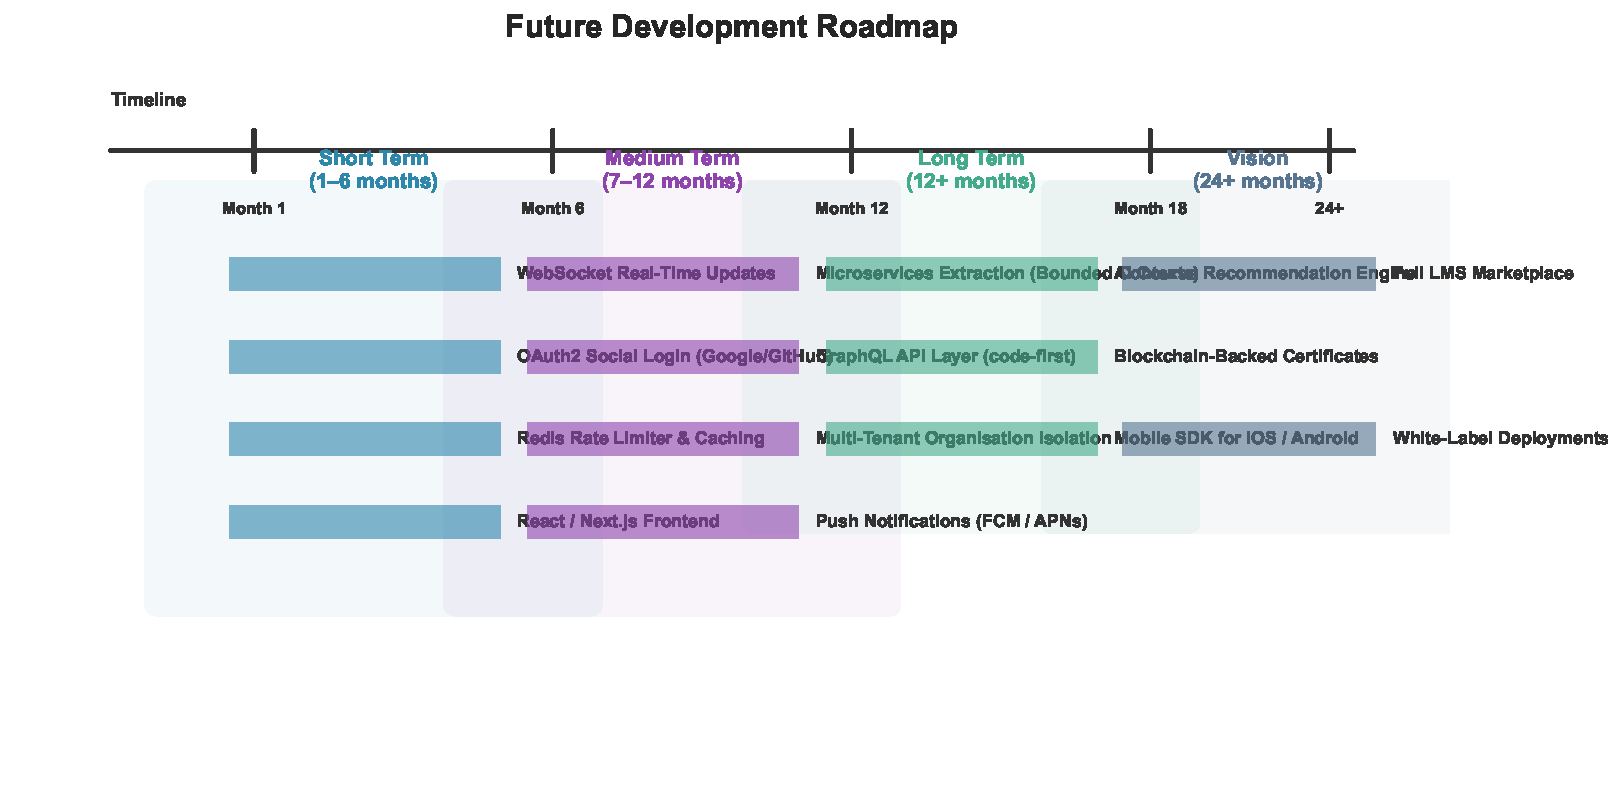
\includegraphics[width=0.85\textwidth]{images/future_work_roadmap.pdf}
  \caption{Priority roadmap for future NexaLearn development, showing short-term (months 1--6), medium-term (months 7--12), and long-term (beyond 12 months) initiatives.}\label{fig:future-roadmap}
\end{figure}
